\documentclass{article}

\usepackage[a4paper,top=3cm,bottom=2cm,left=3cm,right=3cm,marginparwidth=1.75cm]{geometry}
\usepackage[english]{babel}
\usepackage[utf8]{inputenc}
\usepackage{amsmath}
\usepackage{amsfonts}
\usepackage{graphicx}
\usepackage{url}
\usepackage[colorlinks=true, allcolors=blue]{hyperref}

\title{Project: flows on 3D surfaces}
\author{Daw Lara, Pignotti Simone, Revuz Anselme}

\begin{document}
\maketitle

\section*{Introduction}
The goal of the project was to implement different kind of flows for 3D surfaces
using the programming framework Processing, and to compare the results obtained
on multiple surfaces encoded as PLY files. We have implemented the harmonic flow,
the harmonic flow divided by the area, the mean curvature flow and its squared
variant. We also made the computations compatible with open surfaces, for
which the boundary vertices should remain fixed.

\section*{Documentation}
To implement the interface, we used the Processing library G4P. To install it,
open Processing IDE (tested on v3.3.6), go to the ``Sketch'' menu, click on
``Import Library...'', and finally ``Add Library...''. In the window which appears,
search "g4p" in the field ``Filter'' and install ``G4P'' (tested on v4.1.4 of such library).\\

The main menu is composed by three elements:
\begin{itemize}
  \item the ``NEW'' button, allowing to open a new window;
  \item the ``Start/Stop flow'' button, allowing to start or stop the flow on every window;
  \item a list of clickable buttons for opening each window's parameter menu.
\end{itemize}

\begin{center}

\end{center}
\begin{figure}[h]
  \begin{center}
    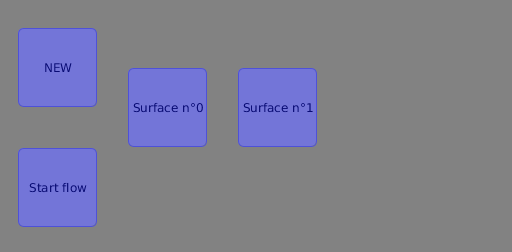
\includegraphics[width=.5\textwidth]{img/main.png}
    \caption{Main menu}
    \label{fig:main}
  \end{center}
\end{figure}

When clicking on the button associated to a window, a new menu appears
allowing to modify the following parameters:
\begin{itemize}
  \item the flow to apply, encoded by an integer, namely:
  \begin{enumerate}
    \item mean curvature with volume renormalization;
    \item mean curvature with projection on the volume constraints;
    \item squared mean curvature with volume renormalization;
    \item squared mean curvature with projection on the volume constraints;
    \item harmonic with volume renormalization;
    \item harmonic with projection on the volume constraints;
    \item harmonic with division by the area and volume renormalization;
    \item harmonic with division by the area and projection on the volume constraints;
  \end{enumerate}
  \item the value of ``tau'', a float $0 < \tau \leq 1$ representing the scaling factor applied to the flow;
  \item the PLY file to use, with examples provided in the data directory;
  \item the activity of the flow on the current window,
    allowing to stop the flow on it even if ``Start flow'' was pressed in the main menu.
\end{itemize}

\begin{figure}[h]
  \begin{center}
    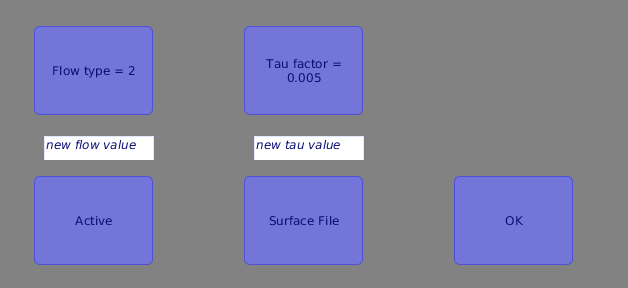
\includegraphics[width=.5\textwidth]{img/win_params.png}
    \caption{Parameters of each window}
    \label{fig:win_params}
  \end{center}
\end{figure}

At creation, a window opens the cube surface, with no flow applied and $\tau = 0.005$.
Once created, the windows cannot be closed. To disable/enable the flow on a window,
click on the ``Active/Inactive'' button.

The value of $\tau$ is parsed as a float, so it is expected to be a floating point
number in the standard notation.

The button ``OK'' allows to go back to the main menu, but every modification
is immediately applied, even without pressing ``OK''.

When a window is selected, the keys 'A' and 'Z' allows to zoom in and out, respectively.

\begin{figure}[h]
  \begin{center}
    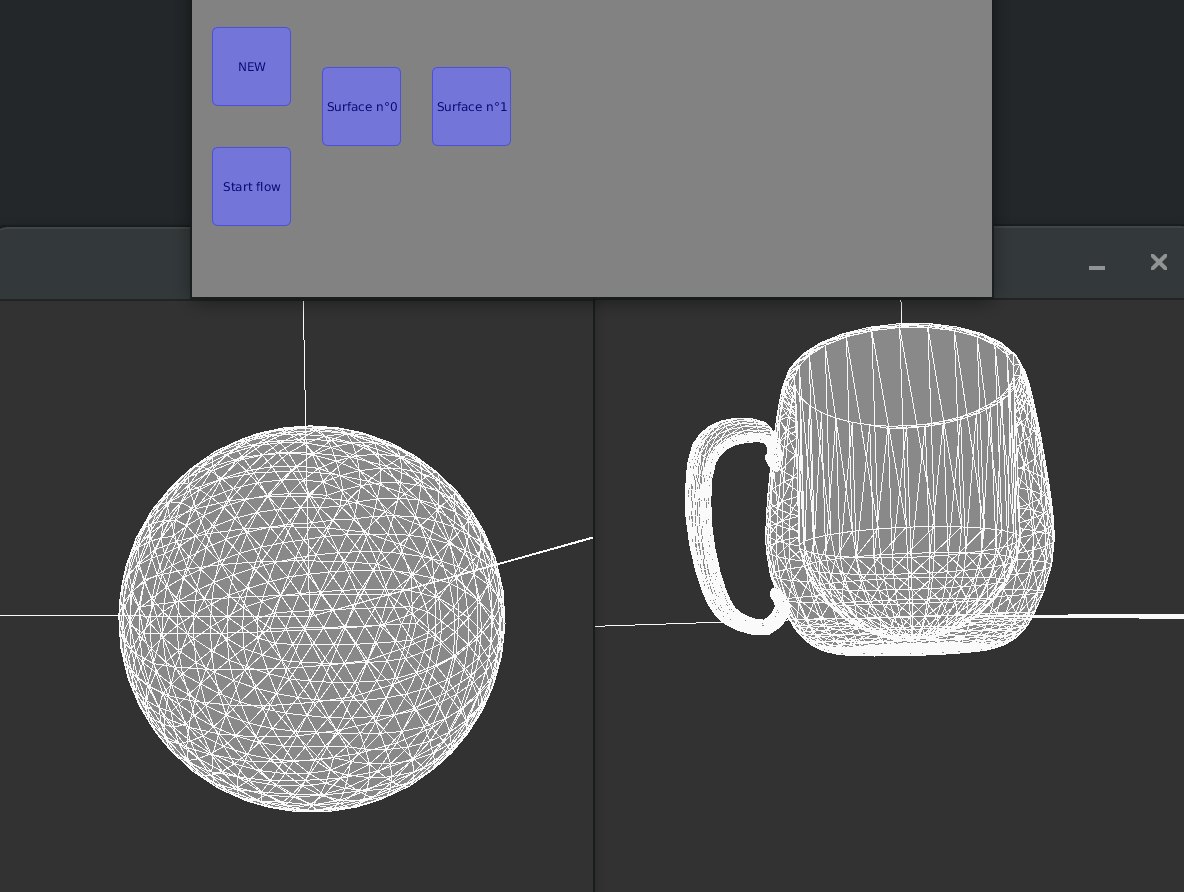
\includegraphics[width=.5\textwidth]{img/mult.png}
    \caption{Multiple windows synchronously applying different flows on different surfaces}
    \label{fig:mult}
  \end{center}
\end{figure}

\section*{Implementation of the flows}

In all the following descriptions, the flow for boundary vertices is set to 0.

\paragraph*{Harmonic Flow:}
For each vertex $p_i$, compute the set of adjacent vertices $N_i$.
For each $p_j \in N_i$, add $p_j$ to $\overrightarrow{H_i}$, and divide by
the cardinality of $N_i$.
\begin{equation*}
  \overrightarrow{H_i}=\frac{1}{|N_i|} \sum_{p_j \in N_i} \overrightarrow{p_j}
\end{equation*}

\paragraph*{Harmonic Area Flow:}
For each vertex $p_i$, compute the set of adjacent vertices $N_i$.
First, calculate the harmonic flow $\overrightarrow{H_i}$ as above, then divide by the area
calculated in the following way:
\begin{equation*}
  A_i = \frac{1}{2} \sum_{j = 1}^{|N_i|} (\overrightarrow{N_i[j] P_i} \times \overrightarrow{N_i[j+1] N_i[j]} )
\end{equation*}
Finally the flow will yield:
\begin{equation*}
  \overrightarrow{H_i}=\frac{1}{A_i} \left( \frac{1}{|N_i|} \sum_{p_j \in N_i} \overrightarrow{p_j} \right)
\end{equation*}

\paragraph*{Mean Curvature Flow:}
Let us define the notation used for each vertex:
\begin{itemize}
  \item $q$ is the point for which the MCF is being computed;
  \item $p_i$ is the predecessor of $q$ on face $j$, the successor of $q$ on face $(j+1)$
    and therefore the shared vertex of faces $(j, j+1)$;
  \item $p_{i-1}$ is the successor of $q$ on face $j$;
  \item $p_{i+i}$ is the predecessor of $q$ on face $(j+1)$;
  \item $\overrightarrow{m_i}$ is the cross product of the edge $(p_i, p_{i+1})$
    by the normal to the plane of $(p_i, q)$ and $(p_{i+1},q)$.
\end{itemize}
Then the following steps are applied:
\begin{itemize}
  \item find the first incident face $f$ and the predecessor and the successor of $q$ in $f$;
  \item iterate over faces containing $q$ in the right order (by finding the face
    containing $q$ and its predecessor;
  \item compute the MCF with the formula:
\end{itemize}
\begin{equation*}
  \overrightarrow{MCF_i} = -\frac{1}{2} \sum_{f \in F : q \in f}
    \overrightarrow{m_i}
\end{equation*}

\paragraph*{Mean Curvature Flow (cotan version):}
This version has been implemented but is not runnable from the main menu.
The other version yields more stable results and is therefore the default choice.

Let us keep the same notation as for the other version, and introduce:
\begin{equation*}
  \alpha_B = \widehat{\overrightarrow{q p_{i-1}} ~ \overrightarrow{p_{i-1} p_{i}}}
\end{equation*}
\begin{equation*}
  \alpha_A = \widehat{\overrightarrow{p_i p_{i+1}} ~ \overrightarrow{p_{i+1} q}}
\end{equation*}
where $B$ stands for ``before'' and $A$ for ``after''. $\overrightarrow{m_i}$ in
this case is the edge $(p_i, q)$. Then:
\begin{itemize}
  \item find the first incident face $f$ and the predecessor and the successor of $q$ in $f$;
  \item Iterate over the faces in the right order by finding the face containing $q$ and its predecessor;
\end{itemize}
Finally, the MCF is given by:
\begin{equation*}
  \overrightarrow{MCF_i} = \frac{1}{2} \sum_{f \in F : q \in f} (\cot{\alpha_B} + \cot{\alpha_A}) \times \overrightarrow{m_i}
\end{equation*}

\paragraph*{Projection on the volume constraints:}
Furthermore, we implemented a method to project any flow on the volume constraints
of the surface and conserve the volume ``a priori'', even for open surfaces.
Of course it is still possible to renormalize ``a posteriori'' by using
the ratio between the initial volume of the surface and the one computed
after having applied the flow.\\
\textit{Step 1:} \textbf{Gradient}\\
For each vertex $p_i$, iterate over the faces to which it belongs and:
\begin{itemize}
  \item find the position of $p_i$ in this face;
  \item iterate over all the vertices other than $p_i$ two by two and calculate their cross product $g_f = \overrightarrow{p_l} \times \overrightarrow{p_k} $.
\end{itemize}
The gradient of $p_i$ is given by $\overrightarrow{G_i} = \sum_{f \in F : p_i \in f} g_f$.\\
\textit{Step 2:} \textbf{Projection}\\
For each vertex $p_i$, the flow $F_i$ will be updated to:
\begin{equation*}
  \hat{F_i} = \overrightarrow{F_i} -
  \frac{\overrightarrow{G_i} \cdot \overrightarrow{F_i}}
    {||\overrightarrow{G_i}||}
  \overrightarrow{G_i}
\end{equation*}

\section*{Examples}
Meaningful examples are given in the form of GIF animations for some of the surfaces.
They can be found in the gifs directory of the repository. They all use the
MCF with different values of $\tau$ on different surfaces:
\begin{itemize}
  \item a sphere with boundary vertices around a pole, with $\tau = 0.01$;
  \item a dodecahedron with $\tau = 0.01$;
  \item a custom surface composed by cubes and half-cubes, with $\tau = 0.01$;
  \item a mug with $\tau = 0.005$.
\end{itemize}

\section*{Conclusions}
The mean curvature flow and its squared variant yield the best results, but
unfortunately none of the implementations manage to keep the original topology of
all surfaces. On complex surfaces, like the mug example, the results are
not as good as expected (no ``smoothing'' effect), but still the computations
are numerically stable enough not to end up in geometrically ill behaviours,
unless the value of $\tau$ is too high.

The biggest improvement was brought by the implementation of the projection
on the volume constraints, which improved the stability of all flows.
A possible improvement is a method to check that vertices do not cross other
faces, but this would add a huge complexity to the calculations, time and space-wise.

\end{document}
